\documentclass[master.tex]{subfiles}
\begin{document}

\chapter{Related Work}

There are many proof assistants available out there, each of them rely on
slightly different meta-theory. We can separate proof assistants into two
categories which are text-base proof assistants and visualised proof assistants.

\section{Text-Base Proof Assistants}

Text-base proof assistants are similar to programming where a user writes
everything in text-files and compiles it; if the compilation is successful, then
the proofs are correct. User can freely manipulate these text-files, hence,
easier to write a complex proof. In addition, most proof assistants have a
plug-in to a mainstream text editor, so users can use their favourite text editor
with full performance.

There are several mainstream text-base proof assistants that are worth
mentioning

\subsection{Coq}
Coq\supercite{coq-official-website} is one the most famous proof assistants. It
is based on the Calculus of Inductive Constructions (CIC)\footnote{CIC is itself
  is developed alongside Coq.} developed by Thierry
Coquand\supercite{thierry-coquand-homepage}.

Coq has customisable tactics which are commands that transform a goal into
smaller-sub goal (if any), this makes proving process become faster compared to
other proof assistants. In contrast, tactics reduce readability, and a reader
might need to replay each tactic step by step in order to understand a proof
completely.

Coq is very mature, it has been developed since 1984. Hence, it is reliable and
has lots of libraries supported.

In term of editor, most people use Proof
General\supercite{proof-general-official-website} which is a plugin on
Emacs\footnote{Proof General also other proof assistants such as Isabelle and PhoX}.
Nevertheless, Coq has its own editor called
CoqIde\supercite{coqide-official-website} that newcomers can use without
learning Emacs.

\begin{figure}[H]
    \centering
    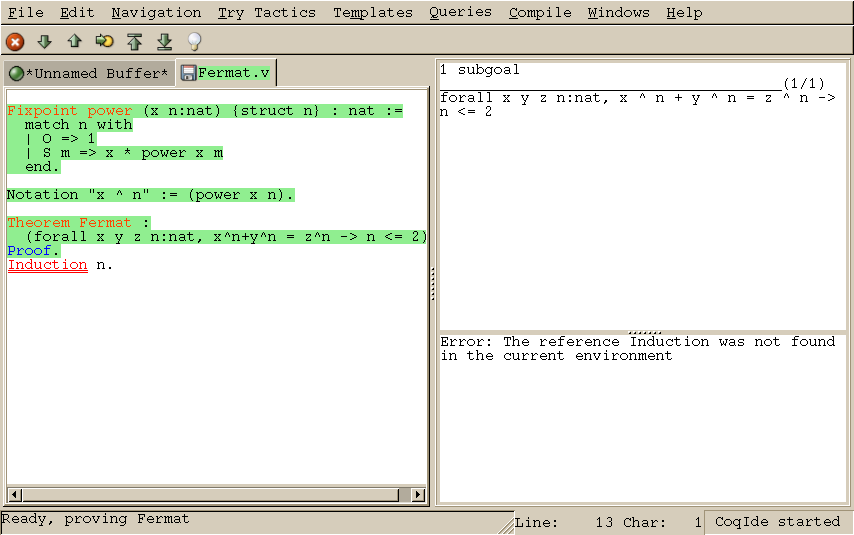
\includegraphics[width=\textwidth]{related-work-coq}
    \caption{Screenshot of Coq (using CoqIde, Credit:
      \cite{coq-official-website}) --- The left pane is file content and Upper
      right pane is the current goal which is changed depending on where the
      cursor point on file content.}
\label{fig:related-work-coq}
\end{figure}

\subsection{Agda}
Adga\supercite{agda-official-website} is (dependently typed) functional
programming which can be seen as a proof assistant as well. It is based on
Unified Theory of Dependent
Types\supercite{norell:thesis}\supercite{Luo:1994:CRT:184757} similar to Martin
Lof Type Theory.

Its proving technique relies on the Curry-Howard correspondence which states
that there is duality between computer programs and mathematical
proofs\supercite{curry-howard-correspondence}; for example functions
corresponded to implication, product types corresponded to logical implication.

Agda is suitable for reasoning about functional programs because we can write a
program and prove that certain properties of a function hold using the same
language. This is feasible since a proof is just a function due to Curry-Howard
correspondence.

Agda has a less steep learning curve compared other proof assistants such as
Coq. This is because users don't need to learn about proving in the system since
it is the same as programming. In contrast, it doesn't have fancy tactic system
so the proving process is slower.

In term of popularity, it is less popular than Coq, however, some projects such
as Homotopy Type Theory\supercite{hott-coq-repo}\supercite{hott-agda-repo} use
Agda as alternative experiments to Coq.

In term of editor, Agda as its own plugin for Emacs which is very nice but user
need to be familiar to Emacs before using it. There is no alternative plugin to
other editor.

\begin{figure}[H]
    \centering
    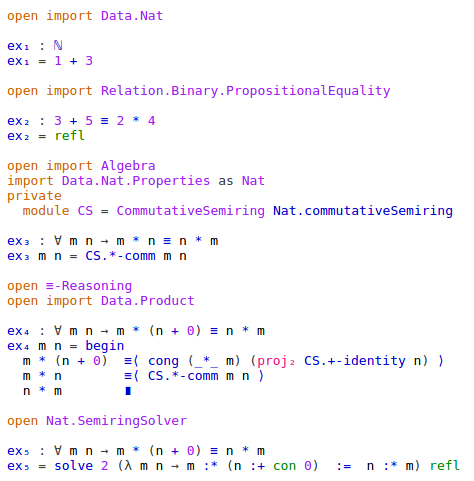
\includegraphics[width=0.6\textwidth]{related-work-agda}
    \caption{Screenshot of Agda --- Credit: an example in Agda standard library,
    removing comment out to save space.}
\label{fig:related-work-agda}
\end{figure}


\subsection{Isabelle}

Isabelle\supercite{isabelle-official-website} is generic proof assistant which
allows user to express mathematical formulae in a formal language and provide a
tool to prove something about it. There are many systems that Isabelle supports
but the most widespread one is \emph{Isabelle/HOL} which provides a higher order
logic environment that is ready for a big application.

One of the main advantages of Isabelle is its readability; the proofs will be
constructed by a language called \emph{Isar} which is designed in such a way
that it can be read easily by both of computers and humans. Another advantage of
Isabelle is that some part of a proof can be automatically proven, this improves
user productivity.

In term of editor, Isabelle has default user interface and Prover IDE called
\emph{Isabelle/jEdit} which is based on jEdit and Isabelle/Scala.

\begin{figure}[H]
    \centering
    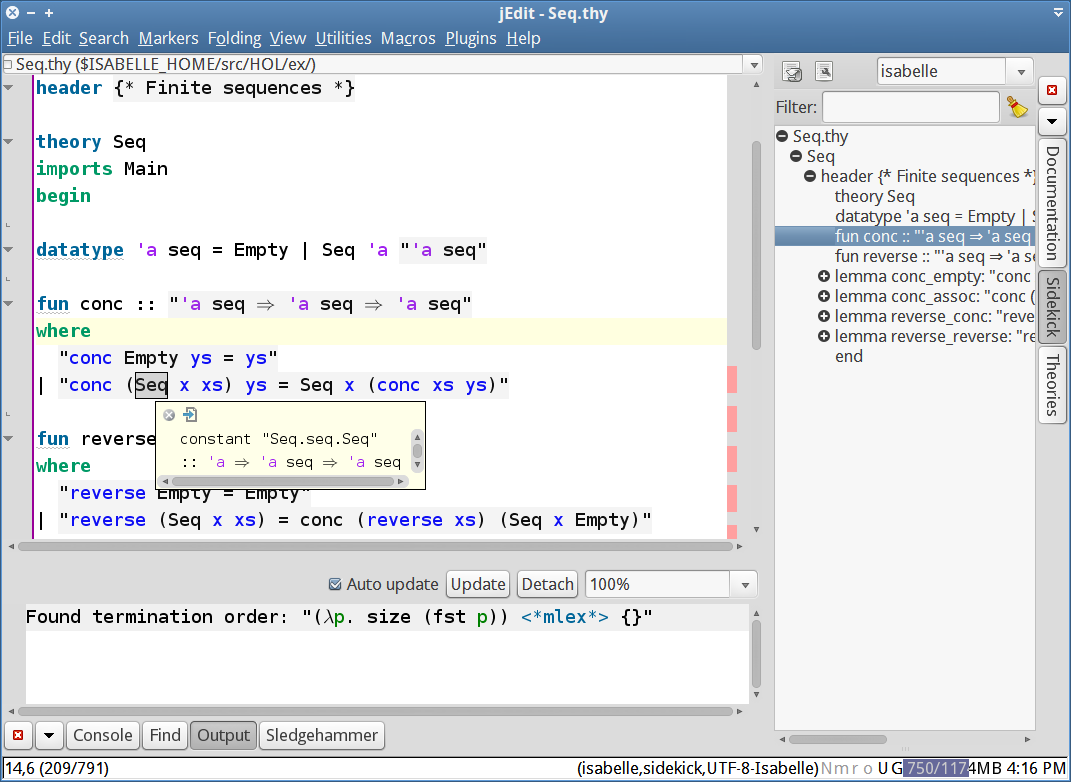
\includegraphics[width=0.8\textwidth]{related-work-isabelle}
    \caption{Screenshot of Isabelle (using Isabelle/jEdit, Credit:
      \cite{isabelle-official-website}) --- The top-left pane shows file content
      and the right pane shows content structure.}
\label{fig:related-work-isabelle}
\end{figure}

\section{Visualised Proof Assistant}
Visualised proof assistants show proofs and related contents in graphical way,
it also allows user to interact with proofs mainly by clicking, which make them
easier to use by newcomers. Nevertheless, users cannot fully manipulate the
proof as they have limited choices of input method, which makes it is harder
have some advance features.

There are much visualised proof assistants out there, so I will show a few of
them to illustrate what visualised proof assistants look like.

\subsection{Logitext}
Logitext\supercite{logitext-official-website} is a web-based proof assistant for
\emph{first-order classical logic} using the \emph{sequent calculus}. The main
intention is to teach students about \emph{Gentzen trees} which is one of a way
to construct a derivation system. Logitext uses Coq internally to check validity
of proof steps.

Logitext is very easy to use, the user usually only needs to click a logical
connector on the goal itself to construct a derivation tree. However, it only
supports sequent calculus for first-order classical logic or propositional
intuitionistic logic and users cannot extend the system.

\begin{figure}[H]
    \centering
    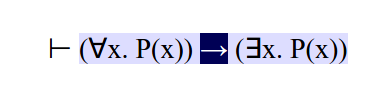
\includegraphics[width=0.5\textwidth]{related-work-logitext-1}
    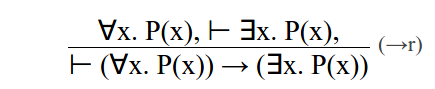
\includegraphics[width=0.6\textwidth]{related-work-logitext-2}
    \caption{Screenshots of Logitext --- You can see that a rule could be invoke
      by just clicking a logical connector.}
\label{fig:related-work-logitext}
\end{figure}

\subsection{Panda}
Panda\supercite{panda-official-website}\supercite{Gasquet2011} (\textbf{P}roof
\textbf{A}ssistant for \textbf{N}atural \textbf{D}eduction for \textbf{A}ll) is
a graphical proof assistant that can be used to prove first order logic using
Gentzen style's natural deduction.

Users interact with it mainly by drag and drop. The main advantage is its
tutorial which is well integrated with the actual program itself.

\begin{figure}[H]
    \centering
    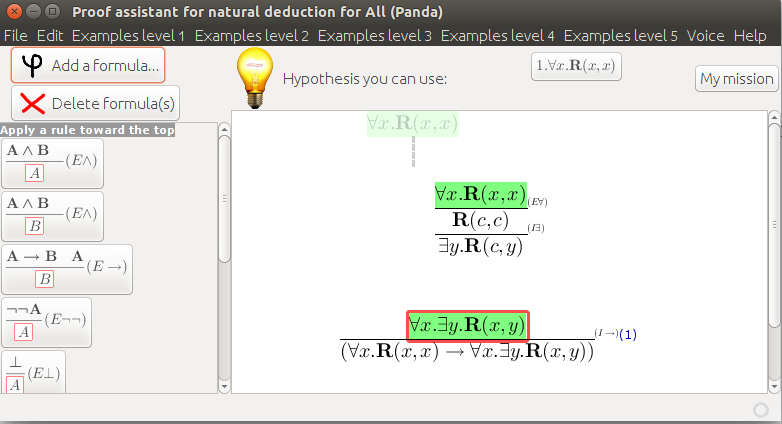
\includegraphics[width=0.8\textwidth]{related-work-panda}
    \caption{Screenshots of Panda --- User can expand the current tree by
      selecting a rule on the left pane and can drag and drop formula around to
      connect it to another one.}
\label{fig:related-work-panda}
\end{figure}

\newpage

\subsection{Pandora}
Pandora\supercite{pandora-official-website}\supercite{Broda2007PandoraAR}
(\textbf{P}roof \textbf{A}ssistant for \textbf{N}atural \textbf{D}eduction using
\textbf{O}rganised \textbf{R}ectangular \textbf{A}reas) is a graphical proof
assistant that can be used to prove first order logic using Fetch style's
natural deduction.

The usage is quite similar to Panda, but it uses boxes (Fetch style) rather than
derivation trees (Gentzen style). It also have a comprehensive document for
newcomers as well.

\begin{figure}[H]
    \centering
    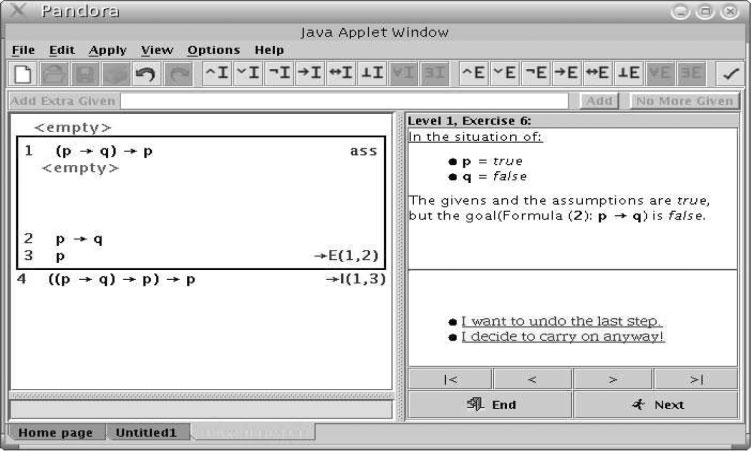
\includegraphics[width=0.8\textwidth]{related-work-pandora}
    \caption{Screenshots of Pandora (Credit: \cite{Broda2007PandoraAR}) ---
      The left pane shows current proof, user can use a rule by clicking on the
      upper pane.}
\label{fig:related-work-pandora}
\end{figure}

\end{document}